% Figure 6 of "Galashin's Conjecture 4.3 via a convex gradient": the three regimes of the window transition.
% Source of the figure, typeset in the paper's own fonts (T1, Latin Modern, 11pt) at the paper's text
% width (6.5in), so \includegraphics does not rescale it. Illustrates CLH-5; it adds no assertion.
% Build: pdflatex <this file> && pdftocairo -svg <this file>.pdf <this file>.svg
\documentclass[11pt]{standalone}
\usepackage[T1]{fontenc}
\usepackage{lmodern}
\usepackage{amsmath,amssymb}
\usepackage{tikz}
\usetikzlibrary{arrows.meta,positioning,calc}

% the palette of the paper's other figures: blue solid for the first strand or arc, ochre dashed for the second
\definecolor{ink}{HTML}{233740}
\definecolor{muted}{HTML}{65757D}
\definecolor{pblue}{HTML}{0072B2}
\definecolor{qochre}{HTML}{B87827}

\tikzset{
  base/.style={draw=muted, line width=0.5pt},
  exit/.style={circle, draw=ink, fill=white, line width=0.6pt, inner sep=0pt, minimum size=4.6pt},
  entry/.style={circle, draw=ink, fill=ink, line width=0.6pt, inner sep=0pt, minimum size=4.6pt},
  exitP/.style={exit, draw=pblue}, entryP/.style={entry, draw=pblue, fill=pblue},
  exitQ/.style={exit, draw=qochre}, entryQ/.style={entry, draw=qochre, fill=qochre},
  strandP/.style={pblue, line width=1.1pt, -{Stealth[length=5pt,width=4.2pt]}, shorten >=2.4pt},
  strandQ/.style={qochre, line width=1.1pt, dash pattern=on 4pt off 1.6pt, -{Stealth[length=5pt,width=4.2pt]}, shorten >=2.4pt},
  lab/.style={font=\footnotesize, inner sep=1.2pt, text=ink},
  labm/.style={font=\small, inner sep=1.2pt, text=ink},
  labP/.style={font=\small, inner sep=1.2pt, text=pblue},
  labQ/.style={font=\small, inner sep=1.2pt, text=qochre},
  muted text/.style={text=muted},
  ttl/.style={font=\small, text=ink, inner sep=0pt},
  negE/.style={font=\small, text=pblue, inner sep=0pt},
  posE/.style={font=\small, text=qochre, inner sep=0pt},
  zeroE/.style={font=\small, text=ink, inner sep=0pt},
  idx/.style={font=\footnotesize, text=muted, inner sep=0pt},
}
\tikzset{
  chA/.style={pblue, line width=1.2pt, -{Stealth[length=6pt,width=5pt]}, shorten >=2.4pt},
  chB/.style={qochre, line width=1.2pt, dash pattern=on 4pt off 1.6pt, -{Stealth[length=6pt,width=5pt]}, shorten >=2.4pt},
  chb/.style={ink, line width=1.2pt, -{Stealth[length=6pt,width=5pt]}, shorten >=2.4pt},
  chr/.style={muted, line width=0.7pt, -{Stealth[length=3.5pt,width=3pt]}, shorten >=2.4pt},
  band/.style={fill=muted!13, draw=none},
  rtitle/.style={font=\small, text=ink, inner sep=0pt, anchor=west},
  fnote/.style={font=\footnotesize, text=ink, inner sep=0pt, anchor=north west, align=flush left},
}
% \chord{style}{x from}{x to}{y}{aspect}: the half-ellipse above the line from the entry to the exit
\newcommand{\chord}[5]{%
  \pgfmathsetmacro{\hx}{abs(#3-#2)/2}\pgfmathsetmacro{\hy}{#5*abs(#3-#2)}%
  \pgfmathparse{int(#2<#3)}%
  \ifnum\pgfmathresult>0
    \draw[#1] (#2,#4) arc[start angle=180, end angle=0, x radius=\hx cm, y radius=\hy cm];%
  \else
    \draw[#1] (#2,#4) arc[start angle=0, end angle=180, x radius=\hx cm, y radius=\hy cm];%
  \fi}

\begin{document}
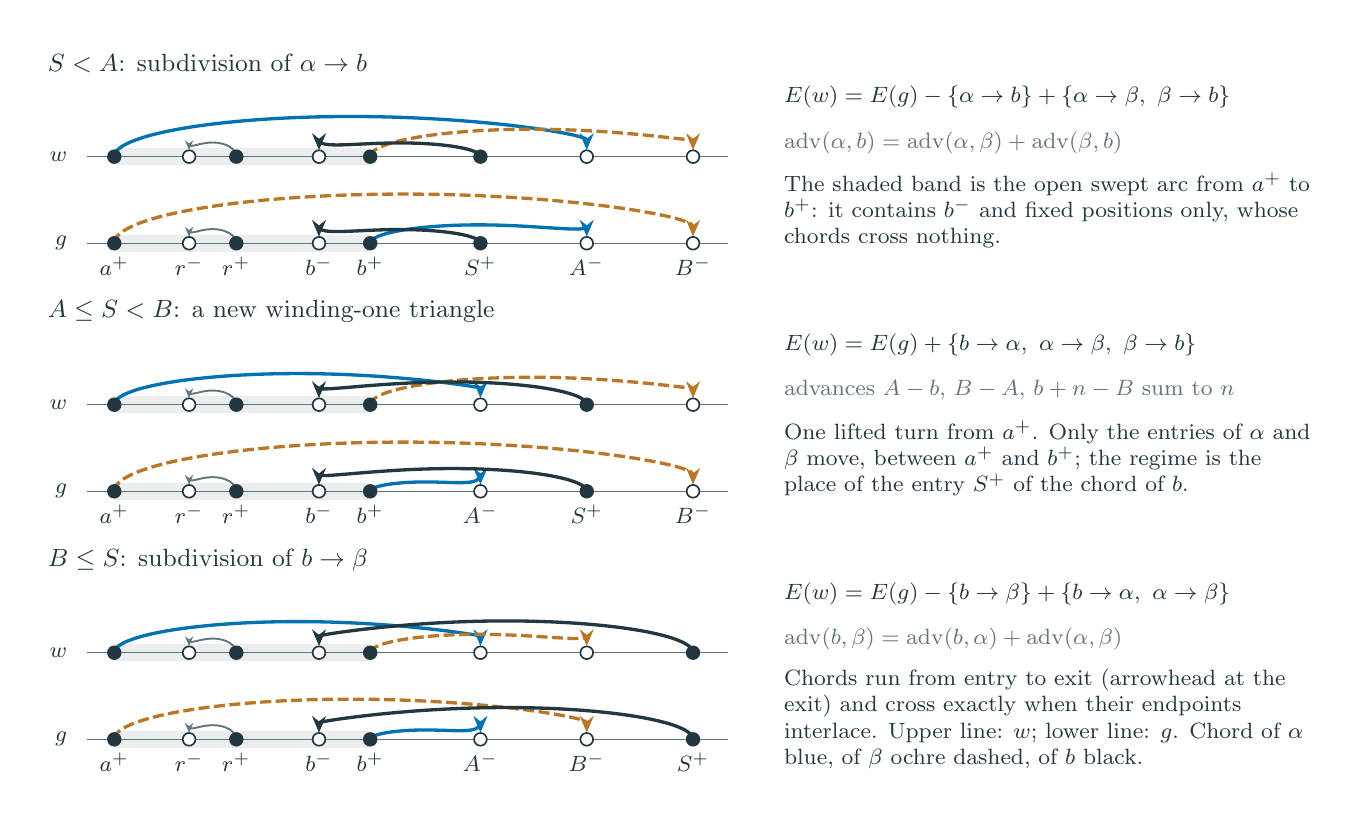
\begin{tikzpicture}[x=1cm,y=1cm]
\useasboundingbox (-0.25000,-9.56800) rectangle (16.26000,0.33800);
\node[rtitle] at (0.0,-0.120) {$S<A$: subdivision of $\alpha\to b$}; %t reg1-title
\fill[band] (0.850,-1.410) rectangle (4.100,-1.190); %band reg1w
\draw[base] (0.5,-1.300) -- (8.65,-1.300);
\node[lab, anchor=east] at (0.300,-1.300) {$w$}; %t reg1w-name
\chord{chr}{2.400}{1.800}{-1.300}{0.3} %k reg1w chr
\chord{chA}{0.850}{6.850}{-1.300}{0.085} %k reg1w chA
\chord{chB}{4.100}{8.200}{-1.300}{0.085} %k reg1w chB
\chord{chb}{5.500}{3.450}{-1.300}{0.085} %k reg1w chb
\node[entry] at (0.850,-1.300) {}; %p reg1w a+
\node[exit] at (1.800,-1.300) {}; %p reg1w r-
\node[entry] at (2.400,-1.300) {}; %p reg1w r+
\node[exit] at (3.450,-1.300) {}; %p reg1w b-
\node[entry] at (4.100,-1.300) {}; %p reg1w b+
\node[entry] at (5.500,-1.300) {}; %p reg1w S+
\node[exit] at (6.850,-1.300) {}; %p reg1w A-
\node[exit] at (8.200,-1.300) {}; %p reg1w B-
\fill[band] (0.850,-2.510) rectangle (4.100,-2.290); %band reg1g
\draw[base] (0.5,-2.400) -- (8.65,-2.400);
\node[lab, anchor=east] at (0.300,-2.400) {$g$}; %t reg1g-name
\chord{chr}{2.400}{1.800}{-2.400}{0.3} %k reg1g chr
\chord{chA}{4.100}{6.850}{-2.400}{0.085} %k reg1g chA
\chord{chB}{0.850}{8.200}{-2.400}{0.085} %k reg1g chB
\chord{chb}{5.500}{3.450}{-2.400}{0.085} %k reg1g chb
\node[entry] at (0.850,-2.400) {}; %p reg1g a+
\node[lab, anchor=north] at (0.850,-2.520) {$a^{+}$}; %t reg1-a+
\node[exit] at (1.800,-2.400) {}; %p reg1g r-
\node[lab, anchor=north] at (1.800,-2.520) {$r^{-}$}; %t reg1-r-
\node[entry] at (2.400,-2.400) {}; %p reg1g r+
\node[lab, anchor=north] at (2.400,-2.520) {$r^{+}$}; %t reg1-r+
\node[exit] at (3.450,-2.400) {}; %p reg1g b-
\node[lab, anchor=north] at (3.450,-2.520) {$b^{-}$}; %t reg1-b-
\node[entry] at (4.100,-2.400) {}; %p reg1g b+
\node[lab, anchor=north] at (4.100,-2.520) {$b^{+}$}; %t reg1-b+
\node[entry] at (5.500,-2.400) {}; %p reg1g S+
\node[lab, anchor=north] at (5.500,-2.520) {$S^{+}$}; %t reg1-S+
\node[exit] at (6.850,-2.400) {}; %p reg1g A-
\node[lab, anchor=north] at (6.850,-2.520) {$A^{-}$}; %t reg1-A-
\node[exit] at (8.200,-2.400) {}; %p reg1g B-
\node[lab, anchor=north] at (8.200,-2.520) {$B^{-}$}; %t reg1-B-
\node[fnote, text width=6.75cm] at (9.35,-0.400) {$E(w)=E(g)-\{\alpha\to b\}+\{\alpha\to\beta,\ \beta\to b\}$}; %t reg1-E
\node[fnote, text width=6.75cm, text=muted] at (9.35,-0.980) {$\operatorname{adv}(\alpha,b)=\operatorname{adv}(\alpha,\beta)+\operatorname{adv}(\beta,b)$}; %t reg1-adv
\node[rtitle] at (0.0,-3.270) {$A\le S<B$: a new winding-one triangle}; %t reg2-title
\fill[band] (0.850,-4.560) rectangle (4.100,-4.340); %band reg2w
\draw[base] (0.5,-4.450) -- (8.65,-4.450);
\node[lab, anchor=east] at (0.300,-4.450) {$w$}; %t reg2w-name
\chord{chr}{2.400}{1.800}{-4.450}{0.3} %k reg2w chr
\chord{chA}{0.850}{5.500}{-4.450}{0.085} %k reg2w chA
\chord{chB}{4.100}{8.200}{-4.450}{0.085} %k reg2w chB
\chord{chb}{6.850}{3.450}{-4.450}{0.085} %k reg2w chb
\node[entry] at (0.850,-4.450) {}; %p reg2w a+
\node[exit] at (1.800,-4.450) {}; %p reg2w r-
\node[entry] at (2.400,-4.450) {}; %p reg2w r+
\node[exit] at (3.450,-4.450) {}; %p reg2w b-
\node[entry] at (4.100,-4.450) {}; %p reg2w b+
\node[exit] at (5.500,-4.450) {}; %p reg2w A-
\node[entry] at (6.850,-4.450) {}; %p reg2w S+
\node[exit] at (8.200,-4.450) {}; %p reg2w B-
\fill[band] (0.850,-5.660) rectangle (4.100,-5.440); %band reg2g
\draw[base] (0.5,-5.550) -- (8.65,-5.550);
\node[lab, anchor=east] at (0.300,-5.550) {$g$}; %t reg2g-name
\chord{chr}{2.400}{1.800}{-5.550}{0.3} %k reg2g chr
\chord{chA}{4.100}{5.500}{-5.550}{0.085} %k reg2g chA
\chord{chB}{0.850}{8.200}{-5.550}{0.085} %k reg2g chB
\chord{chb}{6.850}{3.450}{-5.550}{0.085} %k reg2g chb
\node[entry] at (0.850,-5.550) {}; %p reg2g a+
\node[lab, anchor=north] at (0.850,-5.670) {$a^{+}$}; %t reg2-a+
\node[exit] at (1.800,-5.550) {}; %p reg2g r-
\node[lab, anchor=north] at (1.800,-5.670) {$r^{-}$}; %t reg2-r-
\node[entry] at (2.400,-5.550) {}; %p reg2g r+
\node[lab, anchor=north] at (2.400,-5.670) {$r^{+}$}; %t reg2-r+
\node[exit] at (3.450,-5.550) {}; %p reg2g b-
\node[lab, anchor=north] at (3.450,-5.670) {$b^{-}$}; %t reg2-b-
\node[entry] at (4.100,-5.550) {}; %p reg2g b+
\node[lab, anchor=north] at (4.100,-5.670) {$b^{+}$}; %t reg2-b+
\node[exit] at (5.500,-5.550) {}; %p reg2g A-
\node[lab, anchor=north] at (5.500,-5.670) {$A^{-}$}; %t reg2-A-
\node[entry] at (6.850,-5.550) {}; %p reg2g S+
\node[lab, anchor=north] at (6.850,-5.670) {$S^{+}$}; %t reg2-S+
\node[exit] at (8.200,-5.550) {}; %p reg2g B-
\node[lab, anchor=north] at (8.200,-5.670) {$B^{-}$}; %t reg2-B-
\node[fnote, text width=6.75cm] at (9.35,-3.550) {$E(w)=E(g)+\{b\to\alpha,\ \alpha\to\beta,\ \beta\to b\}$}; %t reg2-E
\node[fnote, text width=6.75cm, text=muted] at (9.35,-4.130) {advances $A-b$, $B-A$, $b+n-B$ sum to $n$}; %t reg2-adv
\node[rtitle] at (0.0,-6.420) {$B\le S$: subdivision of $b\to\beta$}; %t reg3-title
\fill[band] (0.850,-7.710) rectangle (4.100,-7.490); %band reg3w
\draw[base] (0.5,-7.600) -- (8.65,-7.600);
\node[lab, anchor=east] at (0.300,-7.600) {$w$}; %t reg3w-name
\chord{chr}{2.400}{1.800}{-7.600}{0.3} %k reg3w chr
\chord{chA}{0.850}{5.500}{-7.600}{0.085} %k reg3w chA
\chord{chB}{4.100}{6.850}{-7.600}{0.085} %k reg3w chB
\chord{chb}{8.200}{3.450}{-7.600}{0.085} %k reg3w chb
\node[entry] at (0.850,-7.600) {}; %p reg3w a+
\node[exit] at (1.800,-7.600) {}; %p reg3w r-
\node[entry] at (2.400,-7.600) {}; %p reg3w r+
\node[exit] at (3.450,-7.600) {}; %p reg3w b-
\node[entry] at (4.100,-7.600) {}; %p reg3w b+
\node[exit] at (5.500,-7.600) {}; %p reg3w A-
\node[exit] at (6.850,-7.600) {}; %p reg3w B-
\node[entry] at (8.200,-7.600) {}; %p reg3w S+
\fill[band] (0.850,-8.810) rectangle (4.100,-8.590); %band reg3g
\draw[base] (0.5,-8.700) -- (8.65,-8.700);
\node[lab, anchor=east] at (0.300,-8.700) {$g$}; %t reg3g-name
\chord{chr}{2.400}{1.800}{-8.700}{0.3} %k reg3g chr
\chord{chA}{4.100}{5.500}{-8.700}{0.085} %k reg3g chA
\chord{chB}{0.850}{6.850}{-8.700}{0.085} %k reg3g chB
\chord{chb}{8.200}{3.450}{-8.700}{0.085} %k reg3g chb
\node[entry] at (0.850,-8.700) {}; %p reg3g a+
\node[lab, anchor=north] at (0.850,-8.820) {$a^{+}$}; %t reg3-a+
\node[exit] at (1.800,-8.700) {}; %p reg3g r-
\node[lab, anchor=north] at (1.800,-8.820) {$r^{-}$}; %t reg3-r-
\node[entry] at (2.400,-8.700) {}; %p reg3g r+
\node[lab, anchor=north] at (2.400,-8.820) {$r^{+}$}; %t reg3-r+
\node[exit] at (3.450,-8.700) {}; %p reg3g b-
\node[lab, anchor=north] at (3.450,-8.820) {$b^{-}$}; %t reg3-b-
\node[entry] at (4.100,-8.700) {}; %p reg3g b+
\node[lab, anchor=north] at (4.100,-8.820) {$b^{+}$}; %t reg3-b+
\node[exit] at (5.500,-8.700) {}; %p reg3g A-
\node[lab, anchor=north] at (5.500,-8.820) {$A^{-}$}; %t reg3-A-
\node[exit] at (6.850,-8.700) {}; %p reg3g B-
\node[lab, anchor=north] at (6.850,-8.820) {$B^{-}$}; %t reg3-B-
\node[entry] at (8.200,-8.700) {}; %p reg3g S+
\node[lab, anchor=north] at (8.200,-8.820) {$S^{+}$}; %t reg3-S+
\node[fnote, text width=6.75cm] at (9.35,-6.700) {$E(w)=E(g)-\{b\to\beta\}+\{b\to\alpha,\ \alpha\to\beta\}$}; %t reg3-E
\node[fnote, text width=6.75cm, text=muted] at (9.35,-7.280) {$\operatorname{adv}(b,\beta)=\operatorname{adv}(b,\alpha)+\operatorname{adv}(\alpha,\beta)$}; %t reg3-adv
\node[fnote, text width=6.75cm] at (9.35,-1.500) {The shaded band is the open swept arc from $a^{+}$ to $b^{+}$: it contains $b^{-}$ and fixed positions only, whose chords cross nothing.}; %t reg1-band
\node[fnote, text width=6.75cm] at (9.35,-4.650) {One lifted turn from $a^{+}$. Only the entries of $\alpha$ and $\beta$ move, between $a^{+}$ and $b^{+}$; the regime is the place of the entry $S^{+}$ of the chord of $b$.}; %t reg2-intro
\node[fnote, text width=6.75cm] at (9.35,-7.800) {Chords run from entry to exit (arrowhead at the exit) and cross exactly when their endpoints interlace. Upper line: $w$; lower line: $g$. Chord of $\alpha$ blue, of $\beta$ ochre dashed, of $b$ black.}; %t reg3-legend
\end{tikzpicture}
\end{document}
